\documentclass[10pt]{article}
\usepackage{graphicx}
\usepackage{colortbl}
\usepackage{amssymb}
\usepackage{float}
\usepackage{color}
\usepackage{tikz}
\usepackage{xcolor}
\usepackage{epstopdf}
\usepackage{enumitem}
\usepackage{multicol,multirow}
\DeclareGraphicsRule{.tif}{png}{.png}{`convert #1 `dirname #1`/`basename #1 .tif`.png}
\renewcommand{\tablename}{Tabla} 
\renewcommand{\figurename}{Figura} 
\newcommand*\circled[1]{\tikz[baseline=(char.base)]{\node[shape=circle,blue,draw,inner sep=2pt] (char) {#1};}}

\usepackage{listings}

\definecolor{mygreen}{rgb}{0,0.6,0}
\definecolor{mygray}{rgb}{0.5,0.5,0.5}
\definecolor{mymauve}{rgb}{0.58,0,0.82}


\lstset{ %
  backgroundcolor=\color{white},   % choose the background color; you must add \usepackage{color} or \usepackage{xcolor}
  basicstyle=\footnotesize,        % the size of the fonts that are used for the code
  breakatwhitespace=false,         % sets if automatic breaks should only happen at whitespace
  breaklines=true,                 % sets automatic line breaking
  captionpos=b,                    % sets the caption-position to bottom
  commentstyle=\color{gray},       % comment style
  deletekeywords={...},            % if you want to delete keywords from the given language
  escapeinside={\%*}{*)},          % if you want to add LaTeX within your code
  extendedchars=true,              % lets you use non-ASCII characters; for 8-bits encodings only, does not work with UTF-8
  frame=none,	                   % adds a frame around the code
  keepspaces=true,                 % keeps spaces in text, useful for keeping indentation of code (possibly needs columns=flexible)
  keywordstyle=\color{blue},       % keyword style
  language=Java,                 % the language of the code
  otherkeywords={else,open},           % if you want to add more keywords to the set
  numbers=left,                    % where to put the line-numbers; possible values are (none, left, right)
  numbersep=20pt,                   % how far the line-numbers are from the code
  numberstyle=\color{mygray}, % the style that is used for the line-numbers
  rulecolor=\color{black},         % if not set, the frame-color may be changed on line-breaks within not-black text (e.g. comments (green here))
  showspaces=false,                % show spaces everywhere adding particular underscores; it overrides 'showstringspaces'
  showstringspaces=false,          % underline spaces within strings only
  showtabs=false,                  % show tabs within strings adding particular underscores
  stepnumber=2,                    % the step between two line-numbers. If it's 1, each line will be numbered
  stringstyle=\color{mymauve},     % string literal style
  tabsize=2,	                   % sets default tabsize to 2 spaces
  title=\lstname                   % show the filename of files included with \lstinputlisting; also try caption instead of title
}


% For a visual definition of these parameters, see
\textwidth = 6.5 in
\textheight = 9 in
\oddsidemargin = 0.0 in
\evensidemargin = 0.0 in
\topmargin = 0.0 in             
\headheight = 0.0 in            
\headsep = 0.0 in
            
\parskip = 0.2in                % vertical space between paragraphs
% Delete the % in the following line if you don't want to have the first line of every paragraph indented
%\parindent = 0.0in

\begin{document}
\begin{center}
    {\Large Pauta Certamen 3, Programaci\'on II} \\
    \emph{\small Prof. Rodrigo Olivares} \\
    \emph{\scriptsize Enero 4, 2017}
\end{center}
\vspace*{-35pt}
\begin{center}
    \rule{1\textwidth}{.3pt}
\end{center}
\vspace*{-42pt}
\begin{center}
    \rule{1\textwidth}{2pt}
\end{center}

{\scriptsize

\begin{enumerate}

    \item \emph{20pts.} De las siguentes afirmaciones, encierre en un c\'irculo la o las alternativas correctas. Pueden ser todas, algunas, una o ninguna de ellas.
    \begin{multicols}{2}

    \begin{enumerate}[label=(\alph*)]
        \item[i.] Para construir una hebra se requiere:
        \item[\circled{(a)}] Extender de una clase Thread.
        \item[(b)] Implementar una interfaz Thread.
        \item[(c)] Extender de una clase Run.
        \item[(d)] Implementar una interfaz Run.
        \item[(e)] Utilizar el m\'etodo sleep. 
    \end{enumerate}

    \begin{enumerate}[label=(\alph*)]
        \item[ii.] Para una hebra se debe:
        \item[(a)] Iniciar con el m\'etodo run.
        \item[\circled{(b)}] Iniciar con el m\'etodo start.
        \item[\circled{(c)}] Sobreescribir el m\'etodo run.
        \item[(d)] Sobreescribir el m\'etodo start.
        \item[\circled{(e)}] Instanciar la hebra.
    \end{enumerate}

    \begin{enumerate}[label=(\alph*)]
        \item[iii.] En el ciclo de vida de una hebra, el estado: 
        \item[\circled{(a)}] New: crea, pero no inicializa la hebra.
        \item[\circled{(b)}] Runnable: ejecuta la hebra, con tiempo CPU asignado.
        \item[(c)] Blocked: se ejecuta, sin importar estados internos.
        \item[(d)] Dead: es invocado generalmente por el m\'etodo stop.
        \item[\circled{(e)}] Yield, verifica el rendimiento del estado Runnable.
    \end{enumerate}

    \begin{enumerate}[label=(\alph*)]
        \item[iv.] (\emph{3pts.}) Respecto a las interfaces gr\'afica en Java:
        \item Swing sustituye a AWT.
        \item AWT sustituye a Swing.
        \item AWT se apoya en Swing.
        \item AWT incopora los JComponents.
        \item Swing proporciona los ActionEvent.
    \end{enumerate}

    \begin{enumerate}[label=(\alph*)]
        \item[v.] (\emph{3pts.}) Referente a JFrame:
        \item[\circled{(a)}] Habitualmente se usa para crear la ventana principal.
        \item[(b)] Su m\'etodo getPaneContent() obtiene el panel principal.
        \item[\circled{(c)}] Su m\'etodo add() permite agregar componentes al panel.
        \item[(d)] Su m\'etodo size() permite dimensionar la ventana.
        \item[(e)] Todas las anteriores
    \end{enumerate}

    \begin{enumerate}[label=(\alph*)]
        \item[vi.] (\emph{4pts.}) Para las acciones desde un bot\'on, se requiere:
        \item[(a)] Crear una clase que implemente un ActionEvent.
        \item[(b)] Crear una clase que implemente un ActionList.
        \item[(c)] Sobreescribir el m\'etodo actionList(ActionPerformance)
        \item[(d)] Sobreescribir el m\'etodo actionPerformance(ActionEvent)
        \item[\circled{(e)}] Agregar la instancia de la clase oyente, al bot\'on.
    \end{enumerate}
    
\end{multicols}
\newpage

\item \emph{12pts.} Considere el siguiente c\'odigo.

\lstinputlisting[numbers=none,caption=]{java/c3/View.java} 

Describa y diagrame la o las tareas que pueden realizace con esta aplicaci\'on.

\newpage

\begin{multicols}{2}
    
\begin{figure}[H]
    \begin{center}
        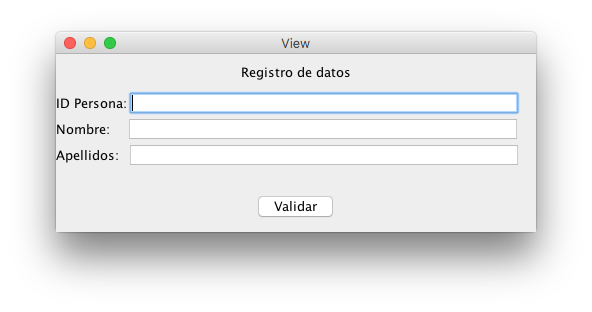
\includegraphics[scale=.45]{images/01.png}
    \end{center}
\end{figure}

\begin{figure}[H]
    \begin{center}
        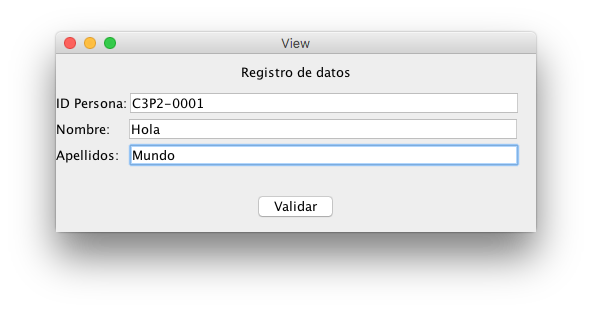
\includegraphics[scale=.45]{images/05.png}
    \end{center}
\end{figure}

\end{multicols}

\begin{multicols}{3}

\begin{figure}[H]
    \begin{center}
        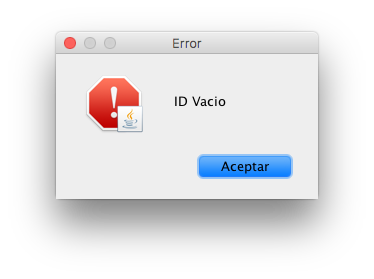
\includegraphics[scale=.5]{images/02.png}
    \end{center}
\end{figure}

\begin{figure}[H]
    \begin{center}
        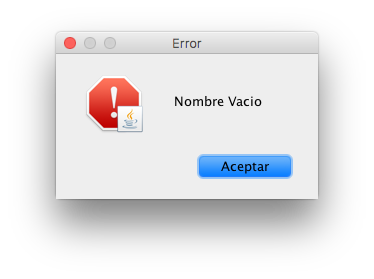
\includegraphics[scale=.5]{images/03.png}
    \end{center}
\end{figure}

\begin{figure}[H]
    \begin{center}
        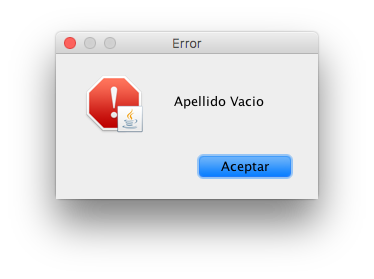
\includegraphics[scale=.5]{images/04.png}
    \end{center}
\end{figure}

\end{multicols}

\textbf{La aplicaci\'on permite ingresar 3 textos: Identificador de una persona, nombre de una persona y apellido de una persona. Si alguno de estos datos no es ingresado, se despliega un mensaje de error.}

\newpage

\item \emph{30pts.} Una empresa de autobuses le ha solicitado a Ud, como alumno de la Escuela de Ingenier\'ia Civil Inform\'atica que desarrolle una simulaci\'on del proceso de subida y bajada de pasajeros. Los requisitos que le impone la empresa son:

\begin{itemize}
    \item La simulaci\'on se realiza s\'olo considerando un autobús
    \item La capacidad m\'axima de un autob\'us es 45 pasajeros (s\'olo se consideran pasajeros sentados).
    \item Si el autob\'us est\'a vac\'io, no puede detenerse para bajar pasajeros.
    \item Si el auto est\'a lleno no puede detenerse para subir pasajeros.
    \item La cantidad de pasajeros que suben y bajan es aleatoria entre 1 y 10.
    \item La frecuencia de subida y bajada de pasajeros es aleatoria en 1 y 5 segundos. 
\end{itemize}

\textbf{Condiciones de entrega:}
\begin{itemize}
    \item[-] \textbf{Debe compilar}. 
    \item[-] Debe considerar la creaci\'on de al menos dos hebras para los proceso y un recurso compartido. 
    \item[-] Subir al aula virtual \textbf{S\'OLO} los archivos \textbf{*.java}, eliminado de ante mano la instrucci\'on \textbf{package}, en un comprimido ApellidoPaternoNombreC3P3.zip. El no cumplimiento del formato ser\'a penalizado con 10 punto de descuento.
    \item[-] Subir a la hora que se les indica en el certamen. El no complimiento con la hora de entrega, ser\'a penalizado con 1 punto de descuento por cada minuto de retraso.
\end{itemize}

\lstinputlisting[numbers=none,caption=]{java/p3/SimulacionAutobus.java} 

\lstinputlisting[numbers=none,caption=]{java/p3/ThreadSubida.java} 

\lstinputlisting[numbers=none,caption=]{java/p3/ThreadBajada.java} 

\lstinputlisting[numbers=none,caption=]{java/p3/Autobus.java} 

\newpage

\item \emph{40pts.} Construya una aplicaci\'on en Java que permita, a trav\'es en una interfaz gr\'afica, realizar la trasnformaci\'on de c\'odigo morse a c\'odigo ASCCI. 

El alfabeto morse es el siguiente:

\begin{table}[H]
    \begin{center}
    \begin{tabular}{|c|c|c|c|c|c|} \hline
      \multicolumn{1}{|>{\columncolor[rgb]{0.8, 0.8, 0.8}}c|}{\textbf{Signo}} &
      \multicolumn{1}{|>{\columncolor[rgb]{0.8, 0.8, 0.8}}c|}{\textbf{C\'odigo}} &
      \multicolumn{1}{|>{\columncolor[rgb]{0.8, 0.8, 0.8}}c|}{\textbf{Signo}} &
      \multicolumn{1}{|>{\columncolor[rgb]{0.8, 0.8, 0.8}}c|}{\textbf{C\'odigo}} &
      \multicolumn{1}{|>{\columncolor[rgb]{0.8, 0.8, 0.8}}c|}{\textbf{Signo}} &
      \multicolumn{1}{|>{\columncolor[rgb]{0.8, 0.8, 0.8}}c|}{\textbf{C\'odigo}} \\ \hline
      A & \textperiodcentered-    & N & -\textperiodcentered & 0 & - - - - -   \\ \hline
      B & -\textperiodcentered\textperiodcentered\textperiodcentered & O & - - -   & 1 & \textperiodcentered- - - -   \\ \hline
      C & -\textperiodcentered-\textperiodcentered & P & \textperiodcentered- -\textperiodcentered & 2 & \textperiodcentered\textperiodcentered- - -   \\ \hline
      D & -\textperiodcentered\textperiodcentered   & Q & - -\textperiodcentered- & 3 & \textperiodcentered\textperiodcentered\textperiodcentered- -   \\ \hline
      E & \textperiodcentered       & R & \textperiodcentered-\textperiodcentered   & 4 & \textperiodcentered\textperiodcentered\textperiodcentered\textperiodcentered-   \\ \hline
      F & \textperiodcentered\textperiodcentered-\textperiodcentered & S & \textperiodcentered\textperiodcentered\textperiodcentered   & 5 & \textperiodcentered\textperiodcentered\textperiodcentered\textperiodcentered\textperiodcentered   \\ \hline
      G & - -\textperiodcentered   & T & -    & 6 & -\textperiodcentered\textperiodcentered\textperiodcentered\textperiodcentered   \\ \hline
      H & \textperiodcentered\textperiodcentered\textperiodcentered\textperiodcentered & U & \textperiodcentered\textperiodcentered-   & 7 & - -\textperiodcentered\textperiodcentered\textperiodcentered   \\ \hline
      I & \textperiodcentered\textperiodcentered     & V & \textperiodcentered\textperiodcentered\textperiodcentered- & 8 & - - -\textperiodcentered\textperiodcentered   \\ \hline
      J & \textperiodcentered- - - & W & \textperiodcentered- -   & 9 & - - - -\textperiodcentered   \\ \hline
      K & -\textperiodcentered-   & X & -\textperiodcentered\textperiodcentered- &  &  \\ \hline
      L & \textperiodcentered-\textperiodcentered\textperiodcentered & Y & -\textperiodcentered- - & & \\ \hline
      M & - -     & Z & - -\textperiodcentered\textperiodcentered &  &  \\ \hline
      
    \end{tabular}
  \end{center}
\end{table}

El c\'odigo ASCII es el siguiente:

    \begin{table}[H]
        \begin{center}
            \begin{tabular}{|c|c|c|c|c|c|} \hline
            \multicolumn{1}{|>{\columncolor[rgb]{0.8, 0.8, 0.8}}c|}{\textbf{Signo}} &
      \multicolumn{1}{|>{\columncolor[rgb]{0.8, 0.8, 0.8}}c|}{\textbf{C\'odigo}} &
      \multicolumn{1}{|>{\columncolor[rgb]{0.8, 0.8, 0.8}}c|}{\textbf{Signo}} &
      \multicolumn{1}{|>{\columncolor[rgb]{0.8, 0.8, 0.8}}c|}{\textbf{C\'odigo}} &
      \multicolumn{1}{|>{\columncolor[rgb]{0.8, 0.8, 0.8}}c|}{\textbf{Signo}} &
      \multicolumn{1}{|>{\columncolor[rgb]{0.8, 0.8, 0.8}}c|}{\textbf{C\'odigo}} \\ \hline
            0&\&\#48; & C&\&\#67; & O&\&\#79;  \\ \hline
            1&\&\#49; & D&\&\#68; & P&\&\#80;  \\ \hline
            2&\&\#50; & E&\&\#69; & Q&\&\#81; \\\hline
            3&\&\#51; & F&\&\#70; & R&\&\#82;  \\\hline
            4&\&\#52; & G&\&\#71; & S&\&\#83;  \\\hline
            5&\&\#53; & H&\&\#72; & T&\&\#84;  \\\hline
            6&\&\#54; & I&\&\#73; & U&\&\#85; \\\hline
            7&\&\#55; & J&\&\#74; & V&\&\#86;  \\\hline
            8&\&\#56; & K&\&\#75; & W&\&\#87;  \\\hline
            9&\&\#57; & L&\&\#76; & X&\&\#88;  \\\hline
            A&\&\#65; & M&\&\#77; & Y&\&\#89;  \\\hline
            B&\&\#66; & N&\&\#78; & Z&\&\#90;  \\\hline
            \end{tabular}
        \end{center}
    \end{table}

\textbf{Restricciomes:}
\begin{itemize}
    \item[-] S\'olo se deben trasnformar palabras que contengan letras may\'usculas y n\'umeros: A-Z y 0-9.
    \item[-] Debe utilizar el paradigma de orientaci\'on a objetos.
\end{itemize}

\textbf{Condiciones de entrega:}
\begin{itemize}
    \item[-] \textbf{Debe compilar}.  
    \item[-] Subir al aula virtual \textbf{S\'OLO} los archivos \textbf{*.java}, eliminado de ante mano la instrucci\'on \textbf{package}, en un comprimido ApellidoPaternoNombreC3P4.zip. El no cumplimiento del formato ser\'a penalizado con 10 punto de descuento.
    \item[-] Subir a la hora que se les indica en el certamen. El no complimiento con la hora de entrega, ser\'a penalizado con 1 punto de descuento por cada minuto de retraso.
\end{itemize}

\newpage

\lstinputlisting[numbers=none,caption=]{java/p4/TransformarMain.java} 

\lstinputlisting[numbers=none,caption=]{java/p4/TransformarView.java} 

\lstinputlisting[numbers=none,caption=]{java/p4/Transformar.java} 

\end{enumerate}
}
\end{document} 
